% !TEX TS-program = XeLaTeX
% Commands for running this example:
% 	 xelatex twocol-example
% 	 xelatex twocol-example
% End of Commands
\documentclass[12pt,twocolumn]{article}

\usepackage{algorithm2e}
\usepackage{url}
\usepackage{tram}
\usepackage{relsize}
\usepackage{amsmath}
\usepackage{float}

\usepackage{xepersian}
\settextfont[Scale=1.1]{B Nazanin}
\setlatintextfont{Georgia}
\DefaultMathsDigits


\newcommand\numberthis[1][]{%
    \refstepcounter{equation}%
    \ifx#1\empty\else\label{eq:#1}\fi%
    \tag{\theequation}%
}
\newcommand{\enfootnote}[1]{\footnote{\lr{#1}}}

\title{ 
\Large{
\textbf{
کاربرد دسته‌بندی کننده‌های مبتنی بر بازنمایی تنک در دسته‌بندی تصاویر
}}}
\date{
\small{
\textbf{
دی ماه 1395
}}}
\author{
\small{
\textbf{
احمد اسدی - ۹۴۱۳۱۰۹۱
}}}

\pagenumbering{arabic}
\begin{document}
\twocolumn[
  \begin{@twocolumnfalse}
%	\begin{figure}[H]
%	\centering
%		
\includegraphics[scale=1]{Imgs/logo.jpg}
%	\end{figure}

    \maketitle
    \begin{abstract}
{\centering
\vspace{10pt}
\begin{tram}[400]
\parbox{\textwidth}{%
دسته‌بندی‌ کننده‌های مبتنی بر بازنمایی تنک عملکرد خوبی در زمینه دسته‌بندی تصاویر، مخصوصا در زمینه دسته‌بندی تصاویر صورت افراد، از خود نشان داده‌اند. به دلیل اهمیت استفاده از چنین دسته‌بندی‌کننده‌هایی، در این گزارش به تفسیر و تبیین این دسته از دسته‌بندی کننده‌ها و معرفی برخی روش‌های بهبود کارایی آن‌ها خواهیم پرداخت. همان‌طور که خواهیم دید، چنین دسته‌بندی‌ کننده‌هایی در مواقعی که داده‌های کلاس‌های مختلف روی یک بردار جهت یکسان توزیع شده باشند، دچار مشکل می‌شود. بنابراین با توسعه این روش با استفاده از یک توسعه غیر خطی، دسته‌بندی کننده‌ای تحت عنوان دسته‌بندی‌ کننده بازنمایی تنک با تابع هسته را که در سال 2012 ارائه شده است، معرفی خواهیم‌نمود. استفاده از توسعه غیرخطی روش بازنمایی تنک، موجب افزایش کارایی مدل شده و امکان ترکیب آن با سایر مدل‌ها را فراهم می‌آورد. به عنوان نمونه مدل ترکیبی از بازنمایی تنک و تطبیق هرم مکانی ارائه شده است که در زمینه دسته‌بندی تصاویر، دقت بالایی را از خود نشان داده است. در انتها روشی را ارائه خواهیم داد که در آن با ترکیب روش یادگیری چندهسته‌ای و بازنمایی تنک، کدهای تنک و وزن‌های هسته در دو مرحله به مدل آموزش داده می‌شوند. این مدل روی مجموعه‌داده‌های مختلفی به منظور دسته‌بندی تصاویر استفاده شده و کارایی خوبی از خود نشان داده است.
}
\end{tram}
}
    \end{abstract}
  \end{@twocolumnfalse}
]

  
\section{مقدمه}    
مفهوم تنک‌بودن\enfootnote{Sparsity} بسته به موضوع پژوهش و بحث می‌تواند معانی مختلفی به خود بگیرد. در زمینه یادگیری ماشین، تنک بودن عموما به مواردی اطلاق می‌شود که در آن‌ها مدل ارائه شده دارای تعداد زیادی مقدار پوچ\enfootnote{Null Values} باشد. با بهره‌گیری از این تعریف، میزان تنک‌بودن را می‌توان با شمارش تعداد ضرایب صفر در بردار پارامترهای مدل، ارزیابی نمود به طوری‌که هر چه تعداد ضرایب صفر موجود در بردار پارامترهای یک مدل افزایش یابد، مدل تنک‌تر می‌شود.
\\
عموما تنک‌بودن در حوزه یادگیری ماشین منجر به افزایش قدرت تعمیم‌پذیری\enfootnote{Generalizability} مدل می‌شود. علاوه بر این، مدل‌های تنک را می‌توان با استفاده از الگوریتم‌هایی با پیچیدگی زمانی پایین‌تر آموزش داد و از آن‌ها استفاده نمود. از این رو وجود چنین خاصیتی در مدل‌ها، مطلوب است.
\\
مقارن با معنای فوق که لزوم توجه به تنک‌بودن مدل را مشخص می‌نماید، می‌توان میزان وابستگی تصمیم‌گیری به داده‌های آموزشی را به عنوان معیار ساده‌ دیگری از تنک‌بودن در نظر گرفت. با فرض این معیار، شباهتی بین این مدل و ماشین‌های بردار پشتیبان\enfootnote{Support Vector Machine (SVM)} وجود خواهد داشت. در مدل ماشین بردار پشتیبان، سعی می‌شود تا حد امکان از تعداد کمتری از داده‌های آموزشی، بردارهای پشتیبان\enfootnote{Support Vectors}، برای برچسب‌دهی و تصمیم‌گیری استفاده شود. در این‌جا نیز هر چه مدل به تعداد کمتری از داده‌های آموزشی وابسته شود، تنک‌تر و مطلوب‌تر است.
\\
استفاده از بازنمایی تنک در دسته‌بندی، از ضرورت یافتن ویژگی‌های مناسب برای دسته‌بندی می‌کاهد. از آنجا که فضای داده‌ها در بازنمایی تنک، یک فضای با ابعاد بسیار بالا است، حتی استفاده از ویژگی‌های تصادفی، اطلاعات کافی را برای دسته‌بندی داده‌ها فراهم می‌آورد و از این طریق فرآیند استخراج ویژگی، که همواره از جمله حساس‌ترین و مهم‌ترین فر‌آیند‌ها در پژوهش‌های مربوط به یادگیری ماشین بوده، تا حد بسیار خوب و قابل توجهی تسهیل می‌یابد.
\\
در پژوهش \cite{wright2009robust} که در سال 2009 ارائه شده است، یک دسته‌بندی کننده مبتنی بر بازنمایی تنک ارائه شده است و از آن در تشخیص چهره استفاده شده است. دسته‌بندی‌کننده مبتنی بر بازنمایی تنک یک مدل ناپارامتری\enfootnote{Nonparametric} فاقد فاز یادگیری است. این مدل قادر است با استفاده از یک مجموعه داده آموزشی که به همراه برچسب صحیح، به مدل داده شده‌اند، مستقیما برچسب مربوط برای داده‌های تست را مشخص نماید.
\\
همان‌طور که در ادامه خواهیم دید، دسته‌بندی‌کننده مبتنی بر بازنمایی تنک ارائه شده توسط رایت و همکارانش در \cite{wright2009robust} در مواردی که بردار توزیع داده‌های دو کلاس، یکسان یا به هم نزدیک باشند، با مشکل در تشخیص روبرو می‌شود. این مشکل به قدری جدی است که مدل ارائه شده حتی در مواردی که داده‌ها به طور خطی جداپذیر باشند در صورتی که شرط مذکور صادق باشد، عملکرد مناسبی از خود نشان نمی‌دهد.
\\
ژنگ و همکارانش در سال 2012 با ارائه پژوهش \cite{zhang2012kernel} و با ترکیب یک تابع هسته با دسته‌بندی‌کننده مبتنی بر بازنمایی تنک، مشکل مدل \cite{wright2009robust} را مرتفع ساختند. استفاده از توابع هسته مختلف، این امکان را می‌دهد که با افزایش بعد داده‌ها و سپس استفاده از یک روش کاهش بعد مناسب، داده‌ها به فضای جدیدی نگاشت شوند که در آن تفکیک‌پذیری داده‌های کلاس‌های مختلف، افزایش بیابد و با ایت کار بتوان مشکل دسته‌بندی‌کننده مبتنی بر بازنمایی تنک را مرتفع ساخت.
\\
ترکیب دسته‌بندی‌کننده مبتنی بر بازنمایی تنک با توابع هسته، امکان انجام فعالیت‌ها و پژوهش‌های مختلف و متنوعی را برای پژوهش‌گران در این زمنیه ایجاد کرده است. از جمله پژوهش‌هایی که با اتکا بر روش‌های پیشین و به منظور ارتقا آن‌ها ارائه شده است می‌توان به پژوهش شریواستاوا و همکارانش در \cite{shrivastava2014multiple} اشاره کرد. در این پژوهش، روشی شامل دو مرحله ارائه شده است که در آن ابتدا با استفاده از یک روش یادگیری، وزن‌های تابع هسته آموزش داده می‌شوند و سپس با استفاده از کد‌های تنک محاسبه شده توسط کرنل آموزش‌دیده، عمل دسته‌بندی انجام می‌شود.
\\
از نمونه‌های دیگر فعالیت‌های مشابه که با اتکا به ترکیب توابع هسته و دسته‌بندی‌کننده‌های مبتنی بر بازنمایی تنک ارائه شده است، پژوهشی است که گائو و همکارانش در سال 2013 در \cite{gao2013sparse} ارائه داده‌اند. در این پژوهش با ترکیب روش تطبیق هرم مکانی و دسته‌بندی‌کننده مبتنی بر بازنمایی تنک با تابع هسته، اقدام به دسته‌بندی تصاویر نموده‌اند.
\\
در ادامه این گزارش، در بخش دوم، ایده اصلی دسته‌بندی‌کننده مبتنی بر بازنمایی تنک را ارائه می‌دهیم. در بخش سوم این گزارش، ایده استفاده از توابع هسته برای افزایش بعد و ترکیب آن با دسته‌بندی‌کننده مبتنی بر بازنمایی تنک را مورد بررسی قرار می‌دهیم. بخش‌های چهارم و پنجم گزارش، به ترتیب به بررسی روش مبتنی بر یادگیری و روش مبتنی بر تطبیق هرم مکانی می‌پردازند. در نهایت یک جمع‌بندی از مطالب ارائه شده در این گزارش و مقایسه نقاط ضعف و قوت روش‌های ارائه شده خواهیم پرداخت.
\\


\section{دسته‌بندی کننده مبتنی بر بازنمایی تنک}
در این بخش به بررسی مدل دسته‌بندی کننده مبتنی بر بازنمایی تنک که رایت و همکارانش در \cite{wright2009robust} ارائه داده‌اند، می‌پردازیم. همان‌طور که قبلا گفته شد، ایده اصلی در این پژوهش، استفاده از ترکیب خطی داده‌های آموزشی برای به دست‌آوردن یک بازنمایی تنک از فضای داده‌ها است. بازنمایی مذکور با استفاده از بهینه‌سازی ریاضیاتی، طوری تعیین می‌شود که کمترین داده‌های آموزشی مورد استفاده قرار بگیرند تا مدل تا حد ممکن تنک شود  و از طرف دیگر خللی در دسته‌بندی داده‌ها ایجاد نشود.
\subsection{تئوری}
با فرض این‌که داده‌های آموزشی از $k$ کلاس مختلف فراهم شده‌اند و تعداد داده‌های آموزشی فراهم شده از کلاس $i$ام را با $n_i$ نمایش دهیم، مجموعه  داده‌های آموزشی کلاس $i$ام را با
 $A_i=\{\nu_{i,1}, \nu_{i,2}, \cdots \nu_{i,n_i}\}$
 نمایش می‌دهیم که $A\in R^{m*n_i}$. از آنجا‌که قصد داریم از این روش در تشخیص چهره استفاده نماییم، داده‌های آموزشی را که تصویر چهره‌ها هستند به شکل یک بردار $\nu \in R^m$ در نظر می‌گیریم که در آن $m = w * h$ و $w$ و $h$ به ترتیب عرض و ارتفاع تصویر را نمایش می‌دهند. به عبارت ساده‌تر تمام پیکسل‌های تصویر را در یک بردار قرار می‌دهیم و از بردارهای حاصل در بقیه فرآیند‌ها استفاده می‌نماییم.
 \\
 با استفاده از ایده اصلی که مطرح شد، می‌توانیم یک تصویر تست $y \in R^m$ را بر اساس داده‌های آموزشی کلاس $i$ام به شکل رابطه \eqref{eq:1-1} مدل‌ کنیم که در آن $\alpha_{i,j}$ ها همگی اعداد حقیقی هستند.
 \begin{equation}
 y = \alpha_{i,1} \nu_{i,1} +\alpha_{i,2} \nu_{i,2} + \cdots +\alpha_{i,n_i} \nu_{i,n_i} 
 \label{eq:1-1}
 \end{equation}
برای این‌که بتوانیم تصویر تست $y$ را بر اساس تمام داده‌های آموزشی مدل کنیم و میزان تعلق آن را به تمام کلاس‌های موجود محاسبه نماییم، ماتریس $A$ را از حاصل کنارهم قرار دادن ماتریس داده‌های آموزشی تمام کلاس‌ها ایجاد می‌نماییم. 
\[
A = [A_1 , A_2 , \cdots, A_k] \in R^{m*N}
\]
که در آن $N = \Sigma_{i=1}^k n_i$ تعداد کل داده‌های آموزشی موجود است. با استفاده از ماتریس $A$ می‌توان رابطه \eqref{eq:1-1} را بر اساس داده‌های آموزشی کلاس $i$ام به شکل رابطه \eqref{eq:1-2} بازنویسی کرد.
\begin{equation}
y = Ax_i
\label{eq:1-2}
\end{equation}

که در آن:
\[
x_i = [0,\cdots,0, \alpha_{i,1}, \alpha_{i,2}, \cdots, \alpha_{i,n_i}, 0 , \cdots, 0]
\]
برداری از تمام ضرایب کلاس $i$ام است.
\\
با استفاده از بازنمایی ارائه شده در \eqref{eq:1-2} داده تست $y$ را به ازای $x_i$های مختلف بازنمایی کرده و از خطای بازسازی\enfootnote{Reconstruction Error} برای تصمیم‌گیری استفاده می‌نماییم. به این معنی که تصویر $y$ را به کلاسی نسبت می‌دهیم که $y - Ax_i$ در آن مقدار کمتری داشته باشد.
\\
از آنجا که بردار $x_i$ مستقیما در برچسب‌دهی تصاویر تست تاثیر دارد، می‌توان مقدار مولفه‌های آن را با استفاده از بهینه سازی مساله خطی $y = Ax_i$ محاسبه نمود. بدون وارد آمدن خللی به مساله می‌توانیم به جای آن که مقادیر مولفه‌های بردار $x_i$ را به ازای $i$های مختلف با بهینه‌سازی بیابیم، مستقیما بردار $x = [x_1,\cdots,x_k]$ را با بهینه‌سازی مساله خطی \eqref{eq:1-3} به‌دست‌ بیاوریم.

\begin{equation}
minimize \>\>\> y = Ax
\label{eq:1-3}
\end{equation}

در صورتی‌که بدانیم $m > n$ است، مساله \eqref{eq:1-3} به یک دستگاه معادلات فرامعین\enfootnote{Overdetermined Equation System} تبدیل می‌شود که می‌توان به طور تحلیلی آن را حل کرد. همین‌طور در صورتی‌که بدانیم $m < n$ است، با یک دستگاه معادلات .....\enfootnote{Underdetermined Equation System} مواجه می‌شویم که پاسخ آن منحصر به فرد نیست. به طور معمول در چنین مواردی با حل مساله نرم۲\enfootnote{$l^2$-norm} مطابق با رابطه \eqref{eq:1-4} و یافتن پاسخ آن، دستگاه معادلات، حل می‌شود.
\begin{align*}
minimize& \>\>\> ||x||_2 \\
subject\>to& \>\>\> y = Ax
\numberthis
\label{eq:1-4}
\end{align*}

روش‌های مختلفی برای حل مساله \eqref{eq:1-4} در زمینه بهینه‌سازی ریاضیاتی وجود دارد. با این وجود پاسخ این مساله، عموما پاسخ مناسبی برای ما نیست به این دلیل که این پاسخ توانایی زیادی در تفکیک داده کلاس‌ها از یک‌دیگر ندارد. آزمایشات نشان می‌دهد پاسخ این مساله، دارای تعداد زیادی ضریب غیر صفر بزرگ از تمام کلاس‌ها است که باعث کاهش قدرت تفکیک‌ داده‌ها توسط مدل می‌شود. 
\\
ایده اصلی روش در حل این مشکل بسیار کارساز است. در شرایطی که تعداد کلاس‌های مساله زیاد باشد، بازنمایی ارائه شده در این پژوهش، یک بازنمایی تنک است که باعث می‌شود تراکم ضرایب غیر صفر در یکی از کلاس‌ها زیاد و در کلاس‌های دیگر نزدیک به صفر باشد که قدرت تفکیک خوبی به مدل می‌دهد. به همین منظور به جای استفاده از تابع نرم۲، از تابع نرم‌صفر\enfootnote{$l^0$-norm} مطابق با \eqref{eq:1-5} استفاده می‌شود.
\begin{align*}
minimize& \>\>\> ||x||_0 \\
subject\>to& \>\>\> y = Ax
\numberthis
\label{eq:1-5}
\end{align*}
تابع نرم‌صفر برابر است با تعداد مولفه‌های غیر صفر یک بردار. با وجود این‌که مساله \eqref{eq:1-5} می‌تواند مشکلات موجود را حل کند، این مساله از جمله مسائل ان‌پی-سخت\enfootnote{NP-hard} است و راه حل سریعی برای حل آن در حالت کلی وجود ندارد. با این حال، می‌توان با درنظر گرفتن شرایط خاص مسائل، راه‌حل‌های خوبی برای آن پیدا کرد.
\\
از طرفی می‌توان پاسخ مساله \eqref{eq:1-5} را در حالتی‌که به دنبال تنک‌ترین پاسخ آن هستیم با مساله بهینه‌سازی نرم۱\enfootnote{$l^1$-norm} مطابق با \eqref{eq:1-6} تخمین بزنیم. همان‌طور که مشخص است در این مساله برای در نظر گرفتن نویزی که به طور معمول در داده‌ها وجود دارد، قید تساوی $y = Ax$ را به $||Ax-y||_2< \epsilon$ تغییر دادیم که در آن $\epsilon > 0$ یک مقدار بسیار کوچک است.

\begin{align*}
minimze& \>\>\> ||x||_1 \\
subject\>to& \>\>\> ||Ax - y||_2 < \epsilon
\numberthis
\label{eq:1-6}
\end{align*}

مساله
 \eqref{eq:1-6}
  با استفاده از برنامه‌ریزی مخروطی مرتبه دوم
  \enfootnote{Second Order Cone Programming}
   قابل حل است و اثبات می‌شود که پاسخ آن به پاسخ
    \eqref{eq:1-5}
     همگرا می‌شود به طوری ‌که ثابت‌های $\rho$ و $\zeta$ وجود خواهند داشت طوری که رابطه \eqref{eq:1-7} را ارضا نمایند.
\begin{equation}
||\hat{x_1} - x_0||_2 \le \zeta \epsilon
\label{eq:1-7}
\end{equation}
که در آن 
$x_0$
 و 
 $x_1$ به ترتیب مقادیر بهینه مسائل \eqref{eq:1-5} و \eqref{eq:1-6} هستند.

\subsection{الگوریتم}
 با ورود یک تصویر تست جدید $y$ ابتدا باید بردار ضرایب را برای این تصویر به دست‌ بیاوریم. این کار را می‌توان با بهینه‌سازی مساله \eqref{eq:1-6} در حالت نویزی یا بدون نویز انجام داد. در مرحله بعد کافیست بردار $x^*$ به‌دست‌آمده را توسط یک دسته‌بندی‌کننده، دسته‌بندی نماییم. این کار می‌تواند در ساده‌ترین حالت به این شکل انجام شود که تصویر ورودی را به کلاس مولفه‌ای از $x^*$ که بیشترین مقدار را دارد تخصیص دهیم.
\\
در این پژوهش به جای استفاده از دسته‌بندی‌کننده مذکور، همان‌طور که قبلا ذکر شد، از خطای بازسازی داده‌ برای دسته‌بندی استفاده می‌نماییم به این معنی که تصویر تست را با ضرایب داده‌های آموزشی همه $k$ کلاس به طور جداگانه بازسازی نموده و خطای بازسازی را محاسبه می‌نماییم و در انتها،‌ تصویر را به کلاسی که کم‌ترین خطای بازسازی را ایجاد نموده است تخصیص می‌دهیم. بازسازی تصویر می‌تواند با استفاده از رابطه \eqref{eq:1-8} برای کلاس $i$ام انجام شود.
\begin{equation}
\hat{y_i} = Ax^*_i
\label{eq:1-8}
\end{equation}
دسته‌بندی‌کننده مذکور را می‌توان مطابق با \eqref{eq:1-9} تریف نمود.
\\
\begin{equation}
min_i r_i(y) = ||y - Ax^*_i||_2
\label{eq:1-9}
\end{equation}


فرآیند توضیح داده شده را می‌توانید در الگوریتم 
\ref{alg:1}
 مشاهده‌ نمایید.
در این الگوریتم ابتدا تمام تصاویر ورودی را که به شکل یک بردار $m$ مولفه‌ای تبدیل شده‌اند، استانداردسازی‌\enfootnote{Normalize}  می‌نماییم به نحوی که نرم۲ همگی آن‌ها برابر با واحد شود. از آن‌جا که خطای نرمال‌سازی را به شکل $||Ax - y||_2$ تعریف نموده‌ایم، این کار باعث می‌شود ضرب داخلی ماتریس $A$ و بردار $x$ دچار مقیاس اندازه نشود. اگر اندازه تصاویر با هم برابر نباشد، این مقیاس اندازه خطای بازسازی را تحت تاثیر قرار داده و موجب می‌شود کلاسی که خطای بازسازی کم‌تری را تولید می‌کند،‌ لزوما بهترین و نزدیک‌ترین کلاس برای تصویر ورودی $y$ نباشد.
\\
در قدم شماره ۳ از الگوریتم \ref{alg:1} مساله نویزی \eqref{eq:1-6} را حل می‌نماییم. برای حل این مساله می‌توان از ابزارهای آماده استفاده نمود. در این پژوهش از کتابخانه حل مسائل برنامه‌ریزی خطی نرم‌افزار مت‌لب\enfootnote{
\url{https://en.mathworks.com/help/optim/ug/linprog.html}
}
استفاده شده است.

در انتها با انتخاب ضرایب هریک از کلاس‌ها و صفر کردن مابقی ضرایب در بردار پاسخ، تصویر ورودی با ترکیب خطی داده‌های هر کلاس متناسب با ضرایب موجود، بازسازی شده و خطای بازسازی آن برای هر کلاس محاسبه می‌شود و کلاسی که کم‌ترین خطای بازسازی را داشته باشد به عنوان برچسب تصویر، انتخاب می‌شود.
\begin{latin}
\begin{algorithm}
 \KwData{a matrix of training samples $A = [A_1, A_2, \cdots, A_k] \in R^{m*n} $ for $k$ classes, test sample $y \in R^m$, error tolerance $\epsilon > 0$} 
 \begin{enumerate}
 \item Normalize the columns of A to have unit $l^2$-norm.
 \item Solve \eqref{eq:1-6} to find $\hat{x}$.
 \item Compute the residuals $r_i(y) = ||y - Ax_i||_2$ for $i = 1, 2, \cdots, k$.
 \end{enumerate}
 \KwResult{$identity(y) = argmin_i r_i(y)$}
 
 \caption{\rl{
 الگوریتم دسته‌بندی با استفاده از دسته‌بندی‌کننده مبتنی بر بازنمایی تنک
 } \cite{wright2009robust}}
 \label{alg:1}
\end{algorithm}
\end{latin}

\subsection{استخراج ویژگی}
برای مدل‌سازی استخراج ویژگی می‌توان از یک ماتریس تبدیل $R$ استفاده کرد. قید تساوی در این حالت به شکل زیر تبدیل می‌شود:
\[
y = RAx , \>\>\> y \in R^d
\]
که در آن $d < n$ است. این تبدیل، تصاویر را از فضای تصاویر به فضای ویژگی‌ها نگاشت می‌کند. پژوهش‌ها نشان‌داده است افزایش بعد فضای ویژگی می‌تواند تاثیر مثبتی در بهبود عملکرد دسته‌بندی‌کننده و افرایش دقت دسته‌بندی داشته باشد. \\
با توجه به این مطلب می‌توانیم مساله \eqref{eq:1-6} را به فرم \eqref{eq:1-10} بازنویسی نماییم.
\begin{align*}
minimize& \>\>\> ||x||_1 \\
subject\>to& \>\>\> ||RAx - y||_2 < \epsilon
\numberthis
\label{eq:1-10}
\end{align*}

مساله‌ای که از اهمیت بالایی برخوردار است، انتخاب مناسب ماتریس $R$ برای دست‌یافتن به دقت‌های دسته‌بندی بالاتر است. نتایج آزمایشات و بررسی‌های ریاضیاتی نشان داده‌اند که در صورتی که تعداد ابعاد فضای ویژگی به طور قابل قبولی زیاد باشد، مطابق با رابطه \eqref{eq:1-11}، می‌توان از یک ماتریس تصادفی برای $R$ استفاده کرد و بهینه‌سازی نرم۱ می‌تواند مقدار بهینه $x^*$ را به خوبی بیابد. 
\begin{equation}
d \ge 2t log(\frac{n}{d})
\label{eq:1-11}
\end{equation}

یکی از نکات بسیار مهم و کاربردی که در این پژوهش می‌توان به آن اشاره کرد این است که:
\begin{center}
«می‌توان از ویژگی‌های تصادفی به منظور دسته‌بندی استفاده کرد که باعث کاهش پیچیدگی فر‌آیند استخراج ویژگی می‌شود.»
\end{center}

\subsection{آزمایشات}

در این بخش آزمایشات مختلفی را که در این پژوهش انجام شده است، مورد بررسی قرار می‌دهیم.
\subsubsection{تاثیر استخراج ویژگی}
در این بخش آزمایشاتی انجام شده است تا تاثیر روش‌های مختلف استخراج ویژگی بر روی عملکرد نهایی دسته‌بندی‌کننده مورد بررسی قرار داده شود.
\\
در آزمایشات این پژوهش از مجموعه داده‌ای\enfootnote{Yale B Database} شامل 2414 تصویر از چهره 38 نفر در شرایط مختلف، انجام شده است. ابعاد همه تصاویر $192 * 168$ است. نیمی از تصاویر به طور تصادفی انتخاب و به عنوان تصاویر آموزشی مورد استفاده قرار گرفته‌اند و مابقی تصاویر به عنوان تصاویر تست استفاده شده‌اند. نتایج آزمایشات روی روش ارائه شده تحت عنوان اس‌آرسی\enfootnote{SRC} و روش‌های نزدیک‌ترین همسایه\enfootnote{NN}، نزدیک‌ترین فضا\enfootnote{Nearest Space (NS)} و ماشین بردار پشتیبان خطی \enfootnote{Linear SVM} اندازه‌گیری و با یک‌دیگر مقایسه شده است. 
\\
در این‌ آزمایش، الگوریتم‌های مختلف با تعداد ابعاد مختلفی از فضای ویژگی مورد استفاده قرار گرفته‌اند. تعداد ابعاد مورد آزمایش در این بخش به ترتیب 30، 56، 120 و 540 بعد بوده است.
\\
شکل \ref{fig:1-1} نتایج مقایسه آزمایشات را نمایش می‌دهد. همان‌طور که در این شکل مشخص است، الگوریتم ارائه شده در مقایسه با روش‌های دیگر به جز روش نزدیک‌ترین فضا، مقاومت بسیار خوبی در برابر تنوع روش‌های انتخاب و استخراج ویژگی از خود نشان داده است. همین‌طور دقت نهایی که الگوریتم به آن دست‌یافته است نسبت به بقیه روش‌ها بالاتر است. از طرفی عمل‌کرد الگوریتم بسیار شبیه به عملکرد الگوریتم نزدیک‌ترین فضا است.
\\
دقت دسته‌بندی کسب‌شده توسط روش اس‌آرسی بین 92.1 تا 95.6 درصد و بیشترین دقت کسب‌شده توسط روش‌های نزدیک‌ترین همسایه، نزدیک‌ترین فضا و ماشین بردار پشتیبان خطی به ترتیب برابر با 90.7، 94.1 و 97.7 درصد بوده است.
\begin{figure*}[h]
\centering
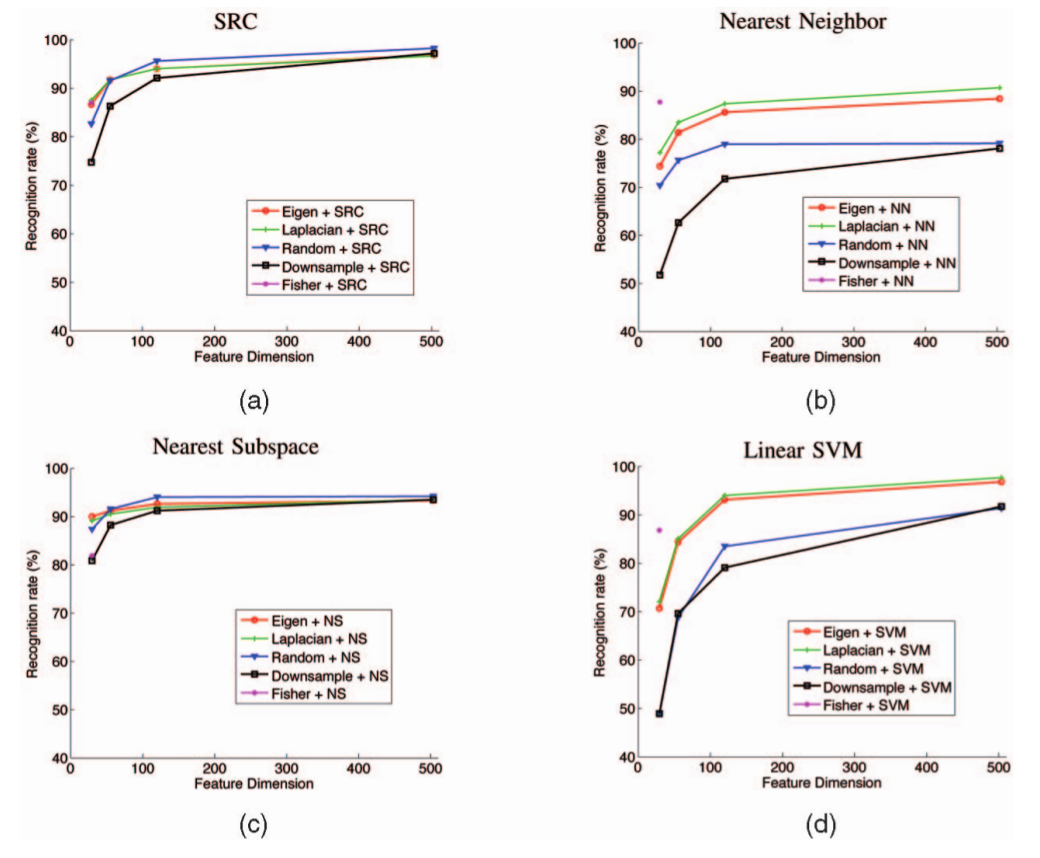
\includegraphics[width=0.8\textwidth]{Imgs/1-1.png}
\caption{نتیجه اعمال روش‌های مختلف استخراج ویژگی بر عملکرد الگوریتم و مقایسه آن با الگوریتم‌های دیگر\cite{wright2009robust}.}
\label{fig:1-1}
\end{figure*}

\subsubsection{استفاده از ویژگی‌های جزئی چهره}
در بسیاری از پژوهش‌ها برای تشخیص چهره از ویژگی‌های جزئی چهره شامل گوش، چشم، بینی، دهان، چانه و انواع اندام‌های دیگر موجود در تصویر چهره استفاده شده است. همین‌طور پژوهش‌های زیادی بر روی نحوه انجام فرآیند تشخیص چهره در مغز انسان با استفاده از همین ویژگی‌های جزئی انجام شده است که باعث بالارفتن اهمیت این موضوع می‌شود.
\\
در این آزمایش هدف، بررسی میزان صحت عملکرد الگوریتم در دسته‌بندی تصاویر و تشخیص چهره با استفاده از ۳ ویژگی بینی، گوش راست و دهان و چانه است. شکل 
\ref{fig:1-2}
 سه ویژگی استخراج شده را برای یک نمونه از تصویر نمایش می‌دهد. نتایج عملکرد الگوریتم‌ها در جدول
  \ref{tbl:1-1}
  ارائه شده است. همان‌طور که در جدول مشاهده می‌شود، عملکرد الگوریتم اس‌آرسی در استفاده از هر ۳ ویژگی نسبت به سایر روش‌ها بهتر بوده است.

\begin{table}[H]
\centering
\caption{جدول نتایج استفاده از الگوریتم‌ها در تشخیص چهره با استفاده از سه ویژگی جزئی چهره\cite{wright2009robust}}
\label{tbl:1-1}
\begin{tabular}{c|c|c|c}
ویژگی‌ها & بینی  & گوش راست‌& دهان و چانه\\
تعداد ابعاد& 4270 & 5040 & 12936 \\
\hline
\hline
\lr{SRC}& 87.3 & 93.7 & 98.3\\
\lr{NN}& 49.2 & 68.8 & 72.7\\
\lr{NS}& 83.7 & 78.6 & 94.4\\
\lr{SVM}& 70.8 & 85.8 & 95.3\\
\end{tabular}
\end{table}

\begin{figure}[H]
\centering
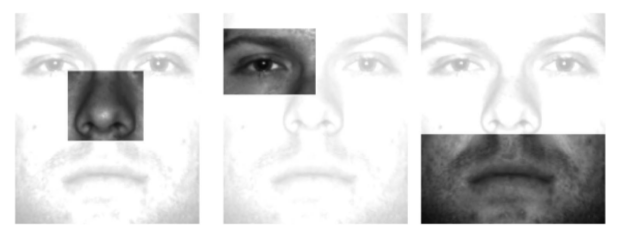
\includegraphics[scale=0.3]{Imgs/1-2.png}
\caption{نمونه‌ای از استخراج سه ویژگی برای یک نمونه از تصاویر\cite{wright2009robust}}
\label{fig:1-2}
\end{figure}


\subsection{تاثیر خرابی تصویر و پوشش بخشی از چهره}
در این آزمایش، میزان تاثیر خرابی بخشی از تصویر در عملکرد دسته‌بندی مورد بررسی قرار می‌گیرد. در مرحله اول از این آزمایش، نویز به بخشی از پیکسل‌های تصویر اعمال می‌شود و در مرحله دوم یک قطعه از تصویر به طور یکپارچه تخریب شده و عملکرد الگوریتم ارزیابی می‌گردد.
\\
جدول \ref{tbl:1-2} نتایج عملکرد الگوریتم را زمانی که درصدی از پیکسل‌های تصویر نویزی می‌شوند نمایش می‌دهد.

\begin{table}[h]
\centering
\caption{عملکرد الگوریتم \lr{SRC} با نویزی کردن درصدی از پیکسل‌های هر تصویر \cite{wright2009robust}}
\label{tbl:1-2}
\begin{tabular}{c|c|c|c}
درصد تخریب&دقت &  درصد تخریب & دقت \\
\hline
\hline
0 & 100 & 50 & 100 \\
10 & 100 & 60 & 99.3 \\
20 & 100 & 70 & 90.7 \\
30 & 100 & 80 & 37.5 \\
40 & 100 & 90 & 7.1
\end{tabular}
\end{table}

همین‌طور شکل \ref{fig:1-3} عملکرد الگوریتم‌های مختلف را بر اساس درصد تخریب تصاویر مورد بررسی قرار می‌دهد. همان‌طور که مشاهده می‌شود الگوریتم اس‌آرسی مقاومت بسیار بالایی نسبت به تخریب تصاویر در مقایسه با روش‌های دیگر از خود نشان می‌دهد.

\begin{figure}[h]
\centering
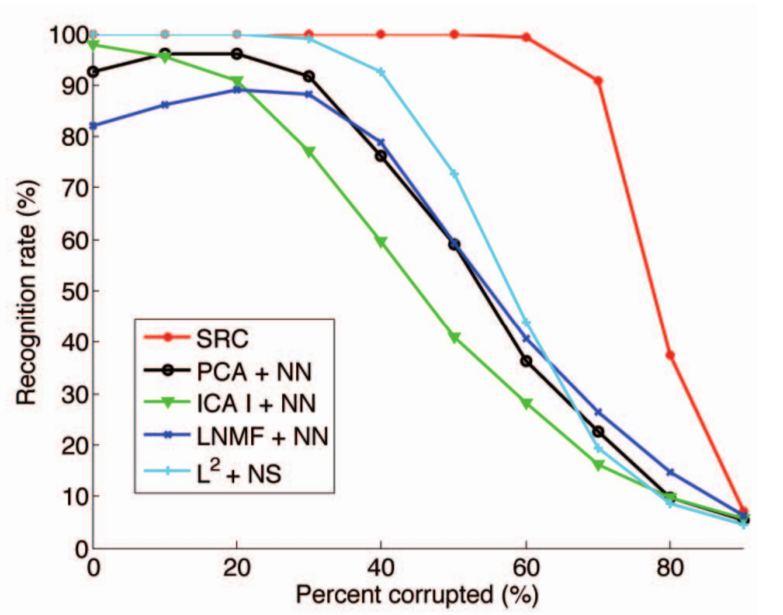
\includegraphics[scale=0.2]{Imgs/1-3.png}
\caption{مقایسه میزان مقاومت الگوریتم‌ها در برابر تخریب تصاویر \cite{wright2009robust}}
\label{fig:1-3}
\end{figure}

به علاوه جدول \ref{tbl:1-3} دقت الگوریتم را در برابر خرابی قطعه‌ای از تصویر گزارش می‌کند. 

\begin{table}[h]
\centering
\caption{عملکرد الگوریتم \lr{SRC} با نویزی کردن قطعه‌ای از هر تصویر \cite{wright2009robust}}
\label{tbl:1-2}
\begin{tabular}{c | c | c | c | c | c }
تخریب&10&20&30&40&50\\
\hline
دقت&100&99.8&98.5&90.3&65.3
\end{tabular}
\end{table}

شکل \ref{fig:1-4} عملکرد الگوریتم را در برابر تخریب قطعه‌ای از تصویر در مقایسه با روش‌های دیگر نمایش می‌دهد که مطابق با آن‌چه در این شکل به نمایش درآمده، مقاومت الگوریتم ارائه شده به مراتب نسبت به الگوریتم‌های دیگر در برابر تخریب قطعه‌ای از تصویر بیشتر است.


\begin{figure}[h]
\centering
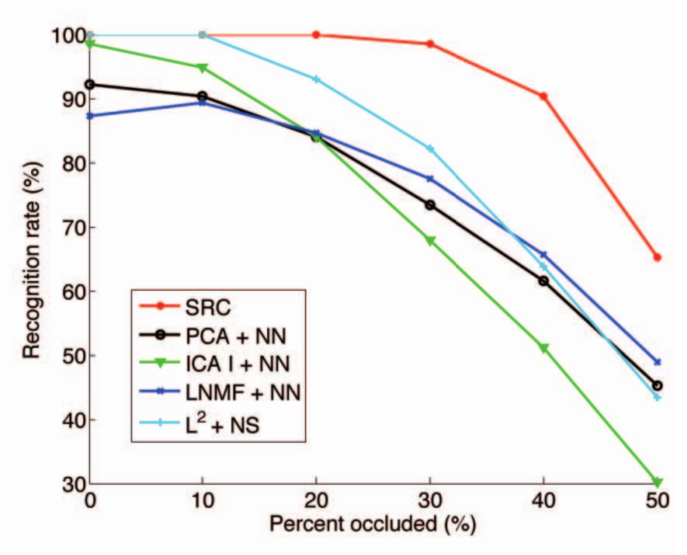
\includegraphics[scale=0.2]{Imgs/1-4.png}
\caption{مقایسه میزان مقاومت الگوریتم‌ها در برابر تخریب قطعه‌ای از تصاویر \cite{wright2009robust}}
\label{fig:1-4}
\end{figure}



\section{دسته‌بندی کننده مبتنی بر بازنمایی تنک با تابع هسته}
همان‌طور که قبلا ذکر شد، دسته‌بندی‌کننده مبتنی بر بازنمایی تنک که در پژوهش \cite{wright2009robust} ارائه شده است، هر تصویر تست را با استفاده از یک ترکیب خطی از داده‌های کلاس‌های موجود بازنمایی کرده و تنک‌ کردن این ترکیب خطی قصد دارد تا شرایطی را فراهم آورد که در آن ضرایب مربوط به داده‌های موجود در نزدیک‌ترین کلاس موجود به تصویر ورودی غیر صفر و مابقی ضرایب صفر شوند.
\\
با توجه به ایده اصلی روش، می‌توان دریافت که در صورتی که داده‌های موجود در مجموعه‌داده آموزشی در دو کلاس مختلف، روی یک بردار جهت یکسان توزیع شده باشند، به طوری‌که بتوان هر یک از داده‌های موجود در یک کلاس را با مقیاس کردن یکی از داده‌های موجود در کلاس دیگر به‌دست آورد، دسته‌بندی‌کننده مبتنی بر بازنمایی تنک،‌ قدرت تفکیک‌ کردن داده‌های این دو کلاس را نخواهد داشت.
\\
برای رفع این مشکل، می‌توان از ایده توابع هسته\enfootnote{Kernel Functions} در یادگیری ماشین استفاده نمود. یک تابع هسته را می‌توان با توجه به قضیه مرسر\enfootnote{Mercer's Theorem} به شکل رابطه \eqref{eq:2-1} نمایش داد.
\begin{equation}
k(x, x^\prime) = \Phi(x)^T\phi(x^\prime)
\label{fig:2-1}
\end{equation}
که در آن، تابع $\Phi$ یک نگاشت غیرخطی و $x$ و $x^\prime$ دو نمونه از داده‌های موجود در مجموعه‌داده هستند. توابع مختلفی ‌می‌توانند با هر تابع هسته مورد استفاده قرار بگیرند. به عنوان مثال‌ می‌توان از تابع گاوسی به عنوان غیرخطی‌کننده تابع هسته استفاده کرد. همین‌طور استفاده از شکل‌های مختلف توابع هسته امکان‌پذیر است.
\\
استفاده از توابع هسته می‌تواند با غیرخطی‌سازی داده‌ها و انتقال آن‌ها به ابعاد بالاتر باعث افزایش تفکیک‌پذیری داده‌ها شده و مشکل روش دسته‌بندی‌کننده مبتنی بر بازنمایی تنک را از بین ببرد.
\\
در این بخش ابتدا تئوری روشی را که توسط ژنگ و همکارانش در \cite{zhang2012kernel} در سال 2012 ارائه شده است، مورد بررسی قرار داده و سپس به بیان الگوریتم روش ترکیبی و آزمایشات انجام شده آن می‌پردازیم.

\subsection{تئوری}
در این روش، سه مرحله وجود دارد که هر یک را به طور جداگانه بررسی می‌نماییم. تصویر ورودی ابتدا در مرحله اول توسط یک تابع هسته از فضای داده به فضای هسته که یک فضا با بعد بالاتر است، نگاشت می‌شود. سپس با به‌کارگیری یک روش مناسب کاهش بعد، فضای هسته به یک فضا با بعد کوچکتر کاهش داده‌ می‌شود. در فضای جدید داده‌ها از تفکیک‌پذری بالاتری نسبت به فضای اولیه برخوردار خواهند بود. سپس عمل دسته‌بندی در فضای جدید انجام می‌شود و برچسب مناسب به تصویر ورودی اختصاص می‌یابد.

\subsubsection{انتقال به فضای هسته}
با فرض این که مساله دارای $c$ کلاس مختلف باشد و تابع غیرخطی‌کننده هسته را با $\Phi$ نمایش دهیم، می‌توانیم برای افزایش تفکیک‌پذیری داده‌ها از یک‌دیگر، تابع غیرخطی‌کننده هسته را به داده‌های اعمال کرده و داده‌ها را به فضای ویژگی‌ها $F$ نگاشت کنیم. این نگاشت مطابق با رابطه \eqref{eq:2-2} انجام می‌شود.
\begin{equation}
\Phi: x \in \Psi \rightarrow \Phi(x) = [\Phi_1(x), \cdots, \Phi_D(x)]^T
\label{eq:2-2}
\end{equation}
همین‌طور می‌دانیم $D >> m$ تعداد ابعاد فضای ویژگی‌ها را مشخص می‌نماید. 
\\
با استفاده از ایده اصلی در روش دسته‌بندی‌کننده مبتنی بر بازنمایی تنک که در آن هر تصویر ورودی را می‌توان با ترکیب خطی از تصاویر آموزشی موجود بازنمایی کرد، در این‌جا هم تصاویر ورودی را می‌توانیم بر اساس یک ترکیب خطی از نگاشت تصاویر آموزشی در فضای ویژگی‌ها بازنمایی بنماییم. این بازنمایی مطابق با رابطه \eqref{eq:2-3} انجام می‌شود.
\begin{equation}
\Phi(y) = \Sigma_{i=1}^n \alpha_i\Phi(x_i) = \Phi\alpha
\label{eq:2-3}
\end{equation}
مطابق با روش دسته‌بندی‌کننده مبتنی بر بازنمایی تنک، می‌توان یک مساله بهینه‌سازی ایجاد کرد که در آن قید تساوی، رابطه \eqref{eq:2-3} باشد. این مساله را با توجه به تمام توضیحاتی که در روش قبل به طور مفصل ارائه شد، از نوع یک مساله بهینه‌سازی نرم۱ انتخاب می‌نماییم. بنابراین، مساله بهینه‌سازی \eqref{eq:2-4} می‌تواند یک بازنمایی مطلوب به ما ارائه دهد.

\begin{align*}
minimize& \>\>\> ||\alpha||_1 \\
subject\>to \>\>\> \Phi(y) = \Phi\alpha
\numberthis
\label{eq:2-4}
\end{align*}

از آن‌جا که ابعاد فضای ویژگی‌ها در مساله \eqref{eq:2-4} بسیار بزرگ‌تر از ابعاد فضای داده است و همین‌طور مدل ارائه شده در \eqref{eq:2-4} در فضای ویژگی‌ها تنک نیست، نمی‌توان به راحتی این مساله را حل نمود. برای حل این مشکلات و یافتن مقدار بهینه این مساله، از روش کاهش بعد با استفاده از توابع هسته استفاده می‌نماییم و این مساله را به یک مساله بهینه‌سازی فضای ممکن\enfootnote{Feasible Optimization Problem} تبدیل می‌نماییم و اقدام به حل آن می‌کنیم.

\subsubsection{کاهش بعد با توابع هسته}

برای اعمال کاهش بعد از فضای ویژگی‌ها، باید یک ماتریس انتقال تعریف نماییم که با ضرب آن در داده‌های موجود در فضای ویژگی‌ها، آن‌ها را به یک فضا با بعد کوچک‌تر نگاشت نماییم. فرض کنیم ماتریس $P\in R^{D*d}$ ماتریس انتقال مناسبی باشد، آن‌گاه برای تبدیل داده‌ها مطابق با رابطه \eqref{eq:2-5} عمل می‌نماییم.

\begin{equation}
P^T\Phi(y) = P^T\Phi\alpha
\label{eq:2-5}
\end{equation}

برای یافتن ماتریس انتقال $P$ با اقتباس از روش‌های $KPCA$ و $KFDA$ از یک ترکیب خطی از داده‌های موجود در مجموعه داده استفاده می‌نماییم. این ماتریس را می‌توانیم مطابق با رابطه \eqref{eq:2-6} محاسبه نماییم.

\begin{equation}
P_j = \Sigma_{i=1}^n \beta_{j,i} \Phi(x_i) = \Phi\beta_j
\label{eq:2-6}
\end{equation}
 که در آن $P_j$ ستون $j$ام از ماتریس انتقال $P$ و $\beta_j = [\beta_{j,1}, \cdots, \beta_{j,n}]^T$ ضرایب ترکیب خطی هستند. بردار $\beta_j$ را بردار شبه انتقال\enfootnote{Pseudo Transformation Vector} مربوط به بردار انتقال $j$ام از ماتریس $P$ می‌نامند. اگر بخواهیم رابطه \eqref{eq:2-6} را در حالت ماتریسی بیان کنیم می‌توانیم از رابطه \eqref{eq:2-7} استفاده نماییم.

\begin{equation}
P = \Phi B
\label{eq:2-7}
\end{equation}
 که در آن $B = [\beta_1, \cdots, \beta_d]^T$ است. اکنون می‌توانیم با جای‌گذاری رابطه \eqref{eq:2-7} در \eqref{eq:2-5} قید تساری را به شکل رابطه \eqref{eq:2-8} بازنویسی نماییم.
 \begin{equation}
 B^Tk(.,y) = B^TK\alpha
 \label{eq:2-8}
 \end{equation}
 که در آن، $k(.,y) = [k(x_1, y), \cdots, k(x_n,y)]^T$ و $K = \Phi^T\Phi$ است. به عبارت دیگر فاصله تحت تابع هسته تمام داده‌های موجود در مجموعه‌آموزشی را با تصویر ورودی، در سمت چپ و فاصله تحت تابع هسته تمام داده‌های آموزشی با یک‌دیگر را در سمت راست قرار می‌دهیم.
 \\
 با توجه به این نکته که با داشتن تابع غیرخطی‌کننده هسته، $k(.,y)$ و $K$ هر دو قابل محاسبه هستند، مساله \eqref{eq:2-4} که قید تساوی آن با \eqref{eq:2-8} جای‌گزین شده باشد، قابل حل می‌شود. در این‌جا ماتریس $B$ نیز به مجموعه متغیرهای مساله اضافه می‌شود.
 \\
  برای محاسبه $B$ می‌توان از یکی از چهار روش زیر بهره گرفت:
  \begin{enumerate}
  \item استفاده از بردارهای ویژه\enfootnote{Eigenvectors} مربوط به بزرگ‌ترین مقادیر ویژه‌\enfootnote{Eigenvalues} کاملا شبیه آن‌چه در روش $KPCA$ از آن استفاده می‌شود. در این روش با محاسبه مقادیر ویژه و انتخاب $d$ مقدار ویژه بزرگ‌تر، بردارهای ویژه مربوط به هریک از مقادیر ویژه انتخاب شده را محاسبه کرده و از کنار هم قرار دادن آن‌ها در ماتریس $B$ به عنوان ماتریس انتقال استفاده می‌نماییم. در این حالت در اصل با استفاده از روش $KPCA$ بعد فضای ويژگی را کاهش می‌دهیم.
  \item با استفاده از روش $KFDA$ می‌توانیم بعد فضای حالت را کاهش دهیم. در این حالت، ماتریس انتقال $B$ پاسخ مساله \eqref{eq:2-9} است.
  \begin{equation}
  maxi_B  \> \> \> \frac{tr(B^TS_b^KB)}{tr(B^TS_w^KB)}
\label{eq:2-9}
  \end{equation}

  \item مطابق با آن‌چه در روش دسته‌بندی‌کننده مبتنی بر بازنمایی تنک ارائه شد، می‌توانیم از یک ماتریس $B$ کاملا تصادفی برای کاهش بعد استفاده نماییم زیرا ماتریس تصادفی نیز اطلاعات کافی برای یافتن پاسخ بهینه مساله بهینه‌سازی نرم۱ با تنک‌ترین پاسخ را دارد. 
  \item همین‌طور می‌توان از یک ماتریس همانی به جای ماتریس $B$ استفاده کرد که در این حالت، کاهش بعدی انجام نمی‌شود. 
  \end{enumerate}
  
  با استفاده از هر یک از چهار روش فوق می‌توان ابعاد فضای ویژگی را کاهش داد.

\subsubsection{دسته‌بندی}
پس از کاهش بعد فضای ویژگی‌ها می‌توانیم اقدام به دسته‌بندی داده‌های ورودی و تست نماییم. مساله بهینه‌سازی که باید حل شود، مطابق با توضیحاتی که ارائه شد، به شکل \eqref{eq:2-10} قابل بیان است.
\begin{align*}
minimize& \>\>\> ||\alpha||_1  \\
subject \> to& \>\>\> B^Tk(.,y) = B^TK\alpha
\numberthis
\label{eq:2-10}
\end{align*}

 با احتساب نویز برای داده‌ها مطابق با روش قبلی، می‌توانیم قید تساوی مساله فوق را تغییر داده و مساله 
 \eqref{eq:2-11}
  را حل نماییم.
  
\begin{align*}
minimize& \>\>\> ||\alpha||_1  \\
subject \> to& \>\>\> ||B^Tk(.,y) - B^TK\alpha||_2 < \epsilon
\numberthis
\label{eq:2-11}
\end{align*} 
 
روند دسته‌بندی در این روش نیز کاملا مطابق با روند دسته‌بندی در روش \lr{SRC} است که قبلا به طور مبسوط شرح داده شد.


\subsection{الگوریتم}

الگوریتم دسته‌بندی‌کننده ارائه شده در \cite{zhang2012kernel} در \ref{alg:2} قابل مشاهده است. همان‌طور که مشاهده می‌شود تمام مراحل این الگوریتم کاملا با مراحل الگوریتم دسته‌بندی‌کننده مبتنی بر بازنمایی تنک یکسان است به جز قسمت‌هایی که مربوط به نگاشت اولیه داده‌ها به فضای ویژگی و سپس کاهش بعد می‌شود. تمام مراحل مطابق با آن‌چه توضیح داده‌ شده است انجام می‌پذیرد. همان‌طور که در این الگوریتم ذکر شده، ابتدا با دریافت تصویر ورودی تست و داده‌های آموزشی می‌توانیم ماتریس‌های $k(.,y)$ و $K$ را مستقیما محاسبه نماییم. این کار در قدم‌های یک و دو انجام شده است. سپس یکی از چهار روش مذکور برای کاهش بعد را انتخاب کرده و ماتریس انتقال آن را محاسبه می‌نماییم. این کار در قدم سوم انجام شده است.


\begin{latin}
\begin{algorithm}
 \KwData{A set of training samples $\{x_i, l_i\}_{i=1}^n$, where $l_i \in \{1,2,\cdots,c\}$, a test sample $y \in R^m$ and an optimal error tolerance $\epsilon > 0$} 
 \begin{enumerate}
 \item Select a kernel $k(.,.)$ and its parameters.
 \item Compute matrix $K = \Phi^T\Phi$ and $k(.,y)$. 
 \item Select a dimensionality reduction method and compute appropriate projection matrix $B$.
 \item Normalize the columns of $B^TK$ and $B^Tk(.,y)$ to have unit $l^2-norm$.
 \item Solve the problem in \eqref{eq:2-11}.
 \item Compute reconstruction errors $r_i(y) = ||B^Tk(.,y) - B^TK\alpha_i||_2$
 \end{enumerate}
 \KwResult{$identity(y) = argmin_i r_i(y)$}
 
 \caption{\rl{
 الگوریتم دسته‌بندی با استفاده از دسته‌بندی‌کننده مبتنی بر بازنمایی تنک ترکیب شده با توابع هسته
 } \cite{zhang2012kernel}}
 \label{alg:2}
\end{algorithm}
\end{latin}


در ادامه با نرمال کردن ستون‌های ماتریس انتقال محاسبه‌شده، تاثیر مقیاس را از خطای بازسازی، چنان‌چه در روش قبلی ذکر شد، از بین می‌بریم. اکنون می‌توانیم مساله مورد نظر را حل نموده و پارامترهای بهینه را برای این مساله محاسبه نماییم. در انتها کلاسی را که کمترین خطای بازسازی را ایجاد نموده است به عنوان برچسب تصویر ورودی، انتخاب نموده و باز می‌گردانیم.

\subsection{آزمایشات}

در این بخش عمل‌کرد روش ارائه شده در \cite{zhang2012kernel} با دسته‌بندی‌کننده مبتنی بر بازنمایی تنک که در \cite{wright2009robust} ارائه شد، مقایسه شده است. در این آزمایش،‌ دو مجموعه داده تستی تولید شده‌اند و با اعمال هر یک از روش‌ها، دقت دسته‌بندی محاسبه و گزارش شده است.
\\
در مجموعه‌داده اول، داده‌های $m$ بعدی از دو کلاس تولید شده‌اند که بازه مقادیر ویژگی‌ها در کلاس اول بین -۳ تا -۱ و در کلاس دوم بین ۱ تا ۳ بوده است. مقادیر مختلف برای $m$ در بازه ۲ تا ۱۲۸ قرار داده‌شده و آزمایش به ازای هر مقدار تکرار شده و نمودارهای شکل \ref{fig:2-2} رسم شده‌اند.
\\
نمودار سمت راست در شکل \ref{fig:2-2} نمایش‌دهنده خطای دسته‌بندی توسط دو دسته‌بندی‌کننده است و همان‌طور که ملاحظه می‌شود، دسته‌بندی‌کننده مبتنی بر بازنمایی تنک قادر به دسته‌بندی نیمی از داده‌ها به طور صحیح است در صورتی‌که دقت دسته‌بندی‌کننده ارائه شده صد در صد است. نمودار سمت راست، ناحیه تصمیم‌گیری دسته‌بندی‌کننده مبتنی بر بازنمایی تنک را نمایش می‌دهد و نمودار وسط، ناحیه تصمیم‌گیری برای دسته‌بندی‌کننده مبتنی بر بازنمایی تنک با ترکیب با توابع هسته را به نمایش گذاشته است. 
\\
همان‌طور که در نمودارهای نمایش داده شده مشخص است، دسته‌بندی‌کننده مبتنی بر بازنمایی تنک با این‌که داده‌ها به طور خطی جداپذیر هستند، قادر به دسته‌بندی داده‌های تولید شده نیست زیرا داده‌های کلاس‌ها روی یک بردار یکسان توزیع شده‌اند.

\begin{figure*}[t]
\centering
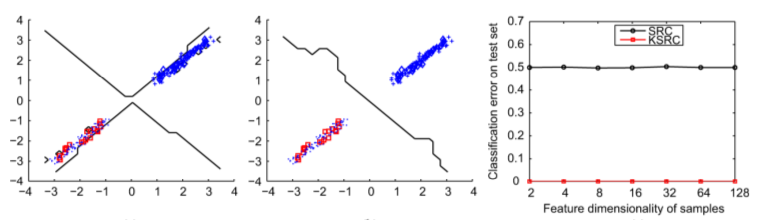
\includegraphics[width=\textwidth]{Imgs/2-2.png}
\caption{نمودار مقایسه عمل‌کرد دسته‌بندی‌کننده مبتنی بر بازنمایی تنک و ترکیب آن با توابع هسته\cite{zhang2012kernel}}
\label{fig:2-2}
\end{figure*}

مجموعه داده دومی که تولید شده است، شامل داده‌های $m$ بعدی از دو کلاس است که دارای توزیع‌های گاوسی متفاوت هستند. ماتریس کوواریانس هر دو کلاس، یک ماتریس همانی است و میانگین‌های آن‌ها با هم متفاوت است.نمودار \ref{fig:2-3} نتیجه آزمایشات را در این حالت برای دو روش فوق، نمایش می‌دهد.

\begin{figure*}[t]
\centering
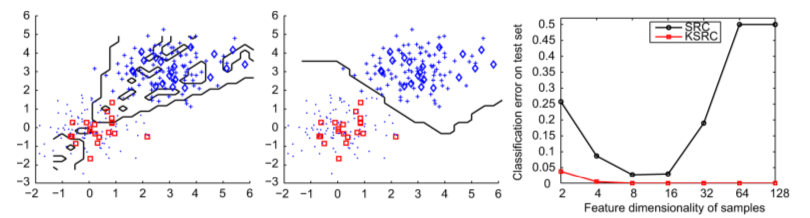
\includegraphics[width=\textwidth]{Imgs/2-3.png}
\caption{نمودار مقایسه عمل‌کرد دسته‌بندی‌کننده مبتنی بر بازنمایی تنک و ترکیب آن با توابع هسته روی داده‌های با توزیع‌های مختلف\cite{zhang2012kernel}}
\label{fig:2-3}
\end{figure*}

محور افقی در نمودار \ref{fig:2-3} تعداد ابعاد فضای ویژگی‌ها را نمایش می‌دهد. همانند آزمایش قبلی، نمودار سمت راست در شکل \ref{fig:2-3} نمایش‌دهنده خطای دسته‌بندی توسط دو دسته‌بندی‌کننده است و همان‌طور که ملاحظه می‌شود، دسته‌بندی‌کننده مبتنی بر بازنمایی تنک عملکرد ضعیفی از خود نمایش داده است مخصوصا با افزایش ابعاد در صورتی‌که دقت دسته‌بندی‌کننده ارائه شده در ابعاد بالاتر به صد در صد رسیده است. نمودار سمت راست، ناحیه تصمیم‌گیری دسته‌بندی‌کننده مبتنی بر بازنمایی تنک را نمایش می‌دهد و نمودار وسط، ناحیه تصمیم‌گیری برای دسته‌بندی‌کننده مبتنی بر بازنمایی تنک با ترکیب با توابع هسته را به نمایش گذاشته است. 

\section{یادگیری وزن‌های تابع هسته}
پژوهش دیگری که در این بخش انجام شده است، پژوهشی است که از ایده دسته‌بندی‌کننده مبتنی بر بازنمایی تنک، در دسته‌بندی اجسام در تصاویر استفاده نموده است. این دسته‌بندی‌کننده، که توسط شریواستاوا و همکارانش در \cite{shrivastava2014multiple} ارائه شده است، با یادگیری تابع هسته سعی در ایجاد بهبود در عملکرد روش‌های پیشین نموده است.

\subsection{تئوری}
همان‌طور که قبلا گفته شد در اصل توابع هسته یک معیاری از میزان شباهت داده‌ها با یک‌دیگر هستند و به نحوی میزان این شباهت را ارزیابی می‌نمایند. از همین رو انتخاب ویژگی‌ها و تابع هسته مناسب در هر مساله از اهمیت بسیاری برخوردار می‌شود. یکی از راه‌های دست‌یابی به چنین روشی، استفاده از ترکیب وزن‌دار تعدادی از توابع هسته از پیش تعریف شده است که موسوم است به روش یادگیری چند هسته‌ای\enfootnote{Multiple Kernel Learning (MKL)}. 
\\
با فرض این‌که $k_1$،  $k_2$ تا $k_M$ توابع هسته از پیش تعریف شده باشند، ترکیب خطی آن‌ها را می‌توانیم مطابق با رابطه \eqref{eq:3-1} تعریف نماییم که در آن ضرایب $\eta_m$ به طور همزمان به طوری که دقت دسته‌بندی را افزایش دهند، با یک‌دیگر یاد گرفته می‌شوند.
\begin{equation}
k(y_i,y_j) = \Sigma_{m = 1}^M \eta_mk_m(y_i,y_j)
\label{eq:3-1}
\end{equation}
 
با اضافه کردن یک شرط دیگر می‌توانیم ترکیب خطی را به طور کنترل‌شده‌تری اعمال کرده و نتایج بهتری دریافت نماییم. در این‌جا شرط \eqref{eq:3-2} را به مساله اضافه می‌نماییم تا بتوانیم یادگیری بهتری روی ضرایب و وزن‌ها داشته باشیم.

\begin{equation}
\Sigma_{i=1}^M \eta_i = 1
\label{eq:3-2}
\end{equation}

اگر دقت دسته‌بندی حاصل از اعمال هسته $k$ام بر مجموعه‌داده را با $\zeta_k$ نمایش دهیم، می‌توانیم دقت حاصل از هسته ترکیبی را مطابق با رابطه  \eqref{eq:3-3} محاسبه نماییم.

\begin{align*}
\zeta &=  \Sigma_{m = 1}^M \eta_mk_m(y_i,y_i) \\
&+ X^T( \Sigma_{m = 1}^M \eta_mk_m(\tilde{Y},\tilde{Y})) X \\
&- 2  \Sigma_{m = 1}^M \eta_mk_m(y_i,\tilde{Y}) X \\
&=  \Sigma_{m = 1}^M \eta_m(k_m(y_i,y_i) \\
&+ X^Tk_m(\tilde{Y},\tilde{Y})X - 2 k_m(y_i,\tilde{Y}) )
\numberthis
\label{eq:3-3}
\end{align*}

که در آن $\tilde{Y}$ مجموعه داده با کنار گذاشتن داده $i$ام است.
\\
با توجه به تابع خطای تعریف شده‌، می‌توانیم با حل مساله بهینه‌سازی \eqref{eq:3-4} وزن‌های بهینه و کدهای تنک $\hat{X}$ را محاسبه نماییم.

\begin{align*}
minimze& \>\>\> \Sigma_{i=1}^N \zeta + \lambda||x_i||_1 \\
subject \> to& \>\>\> \Sigma_{m=1}^M \eta_m = 1 , \eta > 0
\numberthis
\label{eq:3-4}
\end{align*}

دو روش کلی برای حل مساله \eqref{eq:3-4} وجود دارد:
\begin{enumerate}
\item ثابت فرض ‌کردن $\eta$ و حل مساله برای یافتن مقدار $\hat{X}$ بهینه \\
که در این حالت، مساله \eqref{eq:3-4} به یک مساله دسته‌بندی‌کننده مبتنی بر بازنمایی تنک ساده تبدیل می‌شود که قبلا حل شده است.
\item ثابت فرض کردن $\hat{X}$ و حل مساله برای یافتن مقدار $\hat{\eta}$ بهینه \\
در این حالت مساله به یک مساله برنامه‌ریزی خطی\enfootnote{Linear Programming} تبدیل می‌شود که روش‌های متعدد و متنوعی برای حل آن وجود دارد.
\\
با انتخاب این روش، دو مشکل عمده به وجود می‌آید:
\begin{enumerate}
\item تابع هسته یافت شده، تابعی خواهد بود که خطای بازسازی را کاهش می‌دهد و از آن جاکه شرط تنک بودن در آن وجود ندارد، لزوما منجر به دسته‌بندی بهتر نخواهد شد.
\item ترکیب هسته‌ها در هر تکرار، فقط یکی از هسته‌ها را انتخاب می‌کند که باعث ناپایداری شدید الگوریتم می شود.
\end{enumerate}
\end{enumerate}
به منظور حل مشکلات مطرح‌شده، روشی برای ترکیب توابع هسته ارائه می‌شود که در آن تابع هسته طوری تعیین می‌شود که بهترین دسته‌بندی ممکن حاصل شود.
\\
ابتدا تابع امتیازی بین توابع هسته تعریف می‌نماییم. تابع امتیاز بین یک تابع هسته $k_m$ و تابع هسته ایده‌آل $k_d$ را مطابق با رابطه \eqref{eq:3-5} تعریف می‌شود.
\begin{equation}
A_m(k_m, k_d) = \frac{<k_m,k_d>_F}{N\sqrt{<k_m, k_d>_F}}
\label{eq:3-5}
\end{equation}
که در آن:
\[<k_m,k_d>_F = \Sigma_{i=1}^N\Sigma_{j=1}^N k_m(y_i,y_j)k_d(y_i,y_j)\]
و $k_d$ یک ماتریس است که درایه سطر $i$ و ستون $j$ آن برابر یک است اگر $y_i$ و $y_j$ هر دو به یک کلاس تعلق داشته باشند و در غیر این‌صورت برابر صفر خواهد بود.
\\
با تعریف چنین تابع امتیازی می‌توان میزان مناسب بودن یک تابع هسته را ارزیابی نمود. بدون ایجاد خللی در مساله می‌توانیم چنین فرض کنیم :
\[
A_1 > A_2 > \cdots > A_M.
\]
با فرض ثابت بودن $\hat{X}$ می‌توانیم بردار $\hat{\eta}$ را طوری تعیین نماییم که دقت دسته‌بندی افزایش یابد. برای این کار ابتدا خطای دسته‌بندی تابع هسته $m$ام را با تابع $z_i^m$ تعریف می‌نماییم:
\begin{equation}
z_i^m = \left\lbrace \begin{array}{c c}
1, & h_i^m = l_i \\
0, & otherwise
\end{array}\right.
\label{eq:3-6}
\end{equation}
که در آن $h_i^m$ برچسب تشخیص داده‌شده بر اساس تابع هسته $m$ام و $l_i$ برچسب واقعی داده‌ $i$ام است.
معیار ارزیابی صحت عملکرد تابع هسته $m$ام را مطابق با رابطه \eqref{eq:3-7} تعریف می‌نماییم.

\begin{equation}
c_m = \frac{\Sigma_{i:z_i=0}z_i^m}{\Sigma_{i=1}^N (1 - z_i)}
\label{eq:3-7}
\end{equation}

با تعریف معیار \eqref{eq:3-7}، در هر مرحله تابع هسته را مطابق با رابطه \eqref{eq:3-8} انتخاب می‌نماییم که در آن پارامتر $\mu$ پارامتر کنترل‌کننده بیش‌برازش\enfootnote{Overfitting} است.

\begin{equation}
k_{m^*} : \left\lbrace \begin{array}{c c}
c_{m^*} \geq c_m, & m \leq m^* \\
c_{m^*} \geq c_m + \mu, & m > m^* 
\end{array} \right.
\label{eq:3-8}
\end{equation}

وزن مورد استفاده برای ترکیب تابع هسته انتخاب شده بر اساس رابطه \eqref{eq:3-9} محاسبه می‌شود که در آن فقط از داده‌هایی که به اشتباه برچسب‌گذاری شده‌اند استفاده می‌شود.

\begin{equation}
\omega_{m^*} = \frac{\Sigma_{i=1}^N (z_i^{m^*}) \wedge (1-z_i) }{\Sigma_{i=1}^N (1-z_i) \vee (1-z_i^{m^*})}
\label{eq:3-9}
\end{equation}

رابطه \eqref{eq:3-9} نسبت تعداد داده‌هایی را محاسبه می‌کند که تابع هسته جدید قادر به پیش‌بینی برچسب صحیح آن‌ها بوده نسبت به تعداد کل داده‌هایی که تابع هسته کنونی، نتوانسته آن‌ها را به درستی دسته‌بندی نماید. همین‌طور ضریب تاثیر تابع هسته کنونی را مطابق با رابطه \eqref{eq:3-10} محاسبه می‌نماییم.
\begin{equation}
\omega_{curr} = \frac{\Sigma_{i=1}^N (1-z_i^{m^*}) \wedge (z_i) }{\Sigma_{i=1}^N (1-z_i) \vee (1-z_i^{m^*})}
\label{eq:3-10}
\end{equation}
اگر فرض کنیم در تکرار $t$ وزن‌های مورد استفاده برای توابع هسته $\eta^t = [\eta_1^t, \cdots, \eta_M^t]$ بوده باشد، وزن‌های جدید در مرحله بعدی مطابق با رابطه \eqref{eq:3-11} محاسبه می‌شوند.
\begin{equation}
\eta_m^{t+1} = \left\lbrace \begin{array}{c c}
\omega_{m^*} & m = m^* \\
\eta_m^t * \omega_{curr} & otherwise
\end{array}\right.
\label{eq:3-11}
\end{equation}
تمام وزن‌های اولیه برابر با یک مقداردهی می‌شوند و برای استانداردسازی همه وزن‌ها، هر یک از آن‌ها را به مجموع وزن‌ها تقسیم می‌نماییم.


\subsection{الگوریتم}
شبه برنامه روش ارائه شده در \cite{shrivastava2014multiple} در برنامه \ref{alg:3} نمایش داده شده است.



\begin{latin}
\begin{algorithm}
 \KwData{Data samples $Y$, labels $l$, kernel functions $k_m$, parameters $\lambda$ and $\mu$, maximum iteration count $T$, error tolerance $\epsilon_0$} 
\begin{enumerate}
\item for each kernel function $k_m$ and sample $y_i$ compute the predicted label $h_i^m$ by solving the problem \eqref{eq:3-4} and finding the sparse code.
\item initialize $\epsilon_1 \leftarrow \epsilon_0$, $t \leftarrow 0$
\end{enumerate}

\While{$t \leq T$ and $\epsilon_1 \geq \epsilon_0$}
{
  \For {$i = 1,2,\cdots, N$}
%  \State
  {
  Compute $k_m(\tilde(Y_i),\tilde(Y_i))$\;
  Compute the sparse code $x_i$ using \eqref{eq:3-4}\;
  Compute the predicted label $h_i$ using $x_i$\;

  }
%  \EndFor
  Update $\eta_m^t$ for all $m$s \;
  Normalize all weight by computing the sum of all weights and division\;
  Set $\epsilon_1 \leftarrow ||\eta^{t-1} - \eta^t ||_2$\;
  $t \leftarrow t + 1 $ \;
 }
  \KwResult{Kernel function weights $\eta$}
 
 \caption{\rl{
  الگوریتم دسته‌بندی‌کننده مبتنی بر بازنمایی تنک با یادگیری تابع هسته \cite{shrivastava2014multiple}}
 }
 \label{alg:3}
\end{algorithm}
\end{latin}


\subsection{آزمایشات}

با اعمال روش ارائه شده بر مجموعه‌داده شامل تصاویر 128 فرد مختلف به هدف دسته‌بندی تصاویر از لحاظ جنسیت اعمال شده و دقت دسته‌بندی این روش در مقایسه با روش‌های دیگر در جدول \ref{tbl:3-1} مقایسه شده است.

\begin{table}[h]
\centering
\caption{مقایسه دقت عمل‌کرد روش یادگیری توابع هسته با روش‌های دیگر \cite{shrivastava2014multiple}}
\label{tbl:3-1}
\begin{tabular}{c c}
نام روش & دقت\\
\hline
\hline 
\lr{SVM} & 92.4 \\
\lr{NN} & 90.7 \\
\lr{SRC} & 93.0 \\
\lr{KSRC} & 94.1 \\
\lr{MKL-SRC} & 95.4 
\end{tabular}
\end{table}

همین‌طور روش ارائه شده در مقایسه با دسته‌بندی‌کننده مبتنی بر بازنمایی تنک بر روی یک مجموعه‌داده سنتزشده اعمال شده است تا دقت دسته‌بندی این روش با روش‌های دیگر مورد ارزیابی قرار بگیرد. در این پژوهش هم مشکل عدم قدرت تفکیک داده‌های کلاس‌هایی که در یک بردار جهت یکسان توزیع شده باشند در دسته‌بندی‌کننده مبتنی بر بازنمایی تنک، به چالش کشیده شده است. 
\\
در این آزمایش دو مجموعه داده گاوسی با ماتریس کوواریانس یکسان و بردارهای میانگین متفاوت تولید شده و دسته‌بندی شده‌اند. شکل‌\ref{fig:3-1} نتایج این دسته‌بندی را نمایش می‌دهد. شکل اول از سمت راست، نمایش‌دهنده داده‌های تولید شده است. شکل دوم از سمت راست، نگاشت داده‌ها به فضای ویژگی را نمایش می‌دهد. شکل سوم از سمت راست، ناحیه تصمیم‌گیری که توسط روش دسته‌بندی‌کننده مبتنی بر بازنمایی تنک تولید شده است را نمایش داده و شکل چهارم از سمت راست، ناحیه تصمیم‌گیری با روش مبتنی بر تابع هسته را نشان می‌دهد. در نهایت شکل سمت چپ ناحیه تصمیم به‌دست‌آمده توسط روش ارائه شده را نمایش می‌دهد. همان‌طور که در شکل پیداست، قدرت تفکیک داده‌ها در روش جدید به مراتب بالاتر از روش‌های دیگر است.


\begin{figure*}[t]
\centering
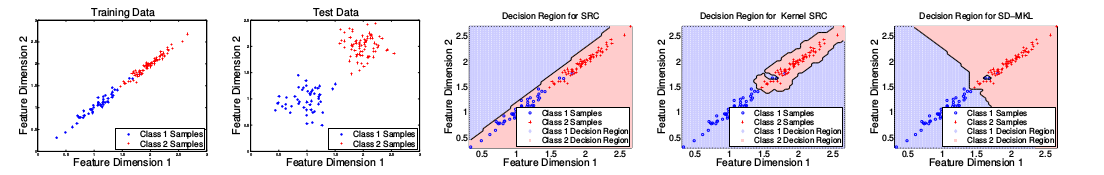
\includegraphics[width=\textwidth]{Imgs/3-1.png}
\caption{مقایسه قدرت دسته‌بندی روش یادگیری توابع هسته با روش پایه \cite{shrivastava2014multiple}}
\label{fig:3-1}
\end{figure*}


\section{استفاده از تطبیق هرم مکانی}



\section{جمع‌بندی و نتیجه‌گیری}
    
    
    
\newpage
\bibliographystyle{ieeetr-fa}
\bibliography{ref}

\end{document} 
